\documentclass[12pt,a4paper]{report}
\usepackage[utf8]{inputenc}
\usepackage[spanish]{babel}
\usepackage{amsmath}
\usepackage{amsfonts}
\usepackage{amssymb}
\usepackage{makeidx}
\usepackage{graphicx}
\usepackage{lmodern}
\usepackage{fourier}
\usepackage[left=2cm,right=2cm,top=2cm,bottom=2cm]{geometry}
\author{Cesar Omar}
\title{EV_1_3_Investigación de par de rotación y cuaternarios}
\begin{document}
Cesar Omar Alvarado Contreras. 6°A
\hspace{3cm}
\includegraphics[scale=.5]{Imagenes/imagen1.png} \\
\\
\\

\textbf{Par de Rotación} \\
Rotación es el movimiento de cambio de rientación de un cuerpo o un sistema de referencia de forma que una lìnea (llamada eje de rotación) o un punto parece fijo.la rotación de un cuerpo se presenta mediante un operador que afecta un conjunto de puntos o vectores.\\
\\
El par motor es el momento de fuerza que ejerce un motor sobre el eje de transmisión de potencia o, dicho de otro modo, la tendencia de una fuerza para girar un objeto alrededor de un eje, punto de apoyo, o de pivote. La potencia desarrollada por el par motor es proporcional a la velocidad angular del eje de transmisión, viniendo dada por:\\x
\\ 
\textbf{P=Mw}\\
\\

Un par de fuerzas es un sistema de dos fuerzas paralelas , de igual intensidad y de sentido contrario, que produce un movimiento de rotación.

Cuando una persona utiliza una llave para quitar la rueda de un automóvil, aplica dos fuerzas iguales y de sentido contrario.\\
\begin{center}
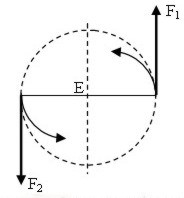
\includegraphics[scale=1]{Imagenes/imagen2.jpg}
\\figura 1.
\end{center}
Se observa que la llave no experimenta movimiento de traslación alguno, es decir, no se desplaza, pero sí gira bajo la acción del par de fuerzas.\\
EL càlculo del par necessario para asegurar la rotacion del conjunto tiene en cuenta:\\
  • las cargas en la maquina\\
   • las masas de arrastre\\
   • las distancias de estas masas respecto al eje de rotacion\\
   • las velociodades y las acelariones\\
   • las pares resistentes\\
\\
Un ejemplo práctio para comprender la diferencia entre par y potencia se puede observar con una bicicleta. Para poder subir una cuesta, a una cierta velocidad, el cicliste debe usar una determinada fuerza en ambos pedales.\\
\\
\begin{center}
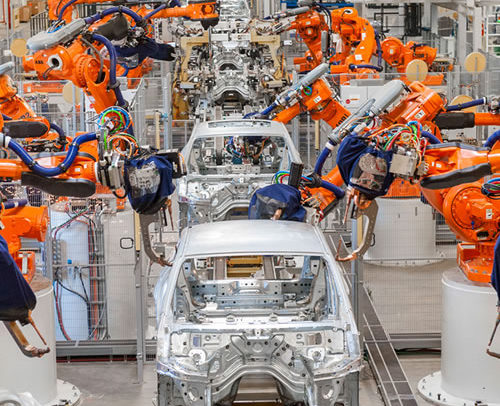
\includegraphics[scale=1]{Imagenes/imagen3.jpg}
\\Figura 2. 
\end{center}
\textbf{Cuaternarios}\\
Los Cuaternarios son las combinaciones entre cuatro elementos distintos, que entran a formar parte de la molécula en la misma o distinta proporciòn, En el caso aplicado a ingenieria o robotica, cuatro elementos mecanicos que formas parte de un sistema mecanico o electrico, y este a su vez comparte acciones y función con otros cuatro sistemas.
\\
Son una extensión de los números reales, similar a la de los números complejos, generada de manera análoga añadiendo las unidades imaginarias.
esto se puede resumir en la siguiente tabla de Cayley.
\begin{center}
Tabla 1.\\
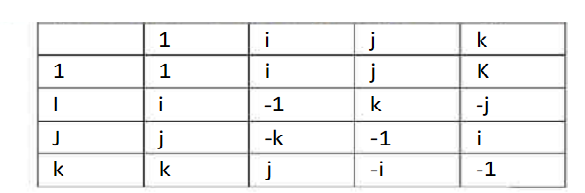
\includegraphics[scale=1]{Imagenes/imagen4.png} 
\end{center}
Entonces se entiende el uso de los cuaternios para localizar un cuerpo rígido en el espacio y conocer la ubicación espacial de sus puntos. En el plano la localización se describe por dos componentes independientes, mientras que en el espacio tridimensional son necesarios tres componentes. Existen diferentes formas de representar la posición en el espacio, la más común es por medio de coordenadas cartesianas o cuaternios.
\\
\end{document}
